\chapter{Layer 2 Scaling: Side Blockchains}
\section{Introduction}

In the recent series of lectures, we have delved into various strategies to enhance the scalability of blockchain systems, addressing aspects like throughput, latency, storage, communication, computation, and energy consumption. In these proposals, a common thread has been the modification of the longest chain consensus protocol. However, making changes to the consensus layer of a practical, operational blockchain system presents significant challenges. Such changes necessitate achieving a "meta consensus" among the participating nodes, essentially agreeing on how to alter the consensus mechanism itself. Even if a successful transition to a new consensus mechanism is achieved, it typically results in a "hard fork" in the ledger, where the blockchain splits into two branches following different consensus protocols.\\
Given this context, the focus of this lecture shifts towards proposals that aim to enhance performance without necessitating changes to the core consensus layer. These proposals operate at what is commonly referred to as "layer 2," where performance scaling is achieved by offloading computation and storage. Importantly, these mechanisms do not compromise the underlying security or integrity of the blockchain system at the "layer 1" level.\\
Among these layer 2 proposals, we'll explore two particularly promising approaches in this lecture: side chains and their ability to support a general account-based model and smart contracts. Side chains offer a means to achieve enhanced performance while maintaining compatibility with the fundamental principles of blockchain technology. This exploration will shed light on how these mechanisms work, their benefits, and how they contribute to the overall scalability and efficiency of blockchain systems.

\section{Side Blockchains}
A side blockchain is essentially a smaller-scale blockchain that represents a subset of trust, often characterized by a reduced number of participating nodes or hash power. This side blockchain is interconnected with a trusted main blockchain through a mechanism where the nodes of the side blockchain periodically commit the cryptographic hashes of their blocks to the main blockchain (as depicted in Figure \ref{fig:L12_f1}a). The ordering of blocks within the side blockchain is determined by the sequence of these committed hashes on the trusted main blockchain. This interconnected structure ensures that the security of the side blockchain is directly derived from the underlying security of the trusted main blockchain.\\
This approach offers a straightforward, practical, and efficient solution. It allows a single trusted main blockchain to efficiently accommodate numerous side blockchains. Unlike a full-fledged blockchain, the trusted main blockchain is not burdened with the need to store, process, or validate the content or semantics of the blocks on the side blockchains. Its role is primarily focused on maintaining and sequencing the hashes associated with these blocks. As a result, this setup enables side blockchains to remain secure and operational even if they lack an honest majority of participants. \\
From a broader perspective, this architecture shares similarities with the concept of a uni-consensus-based sharded blockchain, which was explored in the previous lecture. Both approaches leverage the concept of interconnected blockchains to achieve enhanced scalability and performance, while maintaining security through their connection to a trusted main blockchain.
\begin{center}
	\begin{figure}
		\centering
		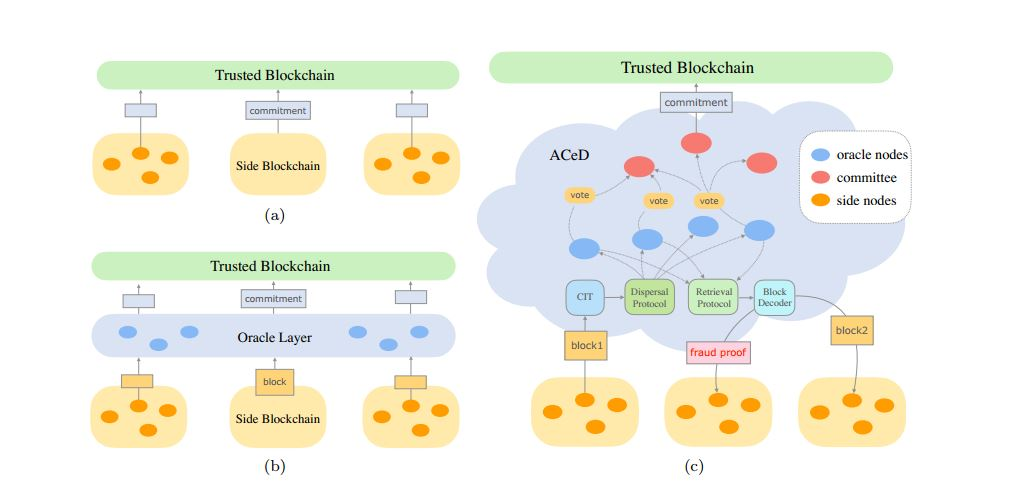
\includegraphics[width=0.8\linewidth]{Fig/12/F1}
		\caption{(a) Side blockchains commit the hashes of blocks to a larger trusted blockchain. (b) An oracle layer is introduced to ensure data availability. (c) ACeD is a scalable data availability oracle.
		}
		\label{fig:L12_f1}
	\end{figure}
\end{center}
\subsection{Data Availability Attack}
The \textit{data availability attack} is a significant vulnerability that affects both the side-blockchain scheme and the sharded blockchain scheme. In this attack, a malicious node within a side blockchain network (or a shard) commits the hash of a block to the trusted main blockchain without actually transmitting the block's data to the other nodes. This creates a dilemma for the users who are trying to construct a coherent ledger from the blockchain: should they wait until they receive the missing block's data, potentially leading to a loss of liveness, or should they proceed without the block's data, risking potential safety violations?\\
The data availability attack was initially introduced in the context of \textit{light clients} in blockchains, as highlighted by Vitalik Buterin of Ethereum in a \href{https://github.com/ethereum/research/wiki/A-note-on-data-availability-and-erasure-coding}{note} and an \href{https://arxiv.org/abs/1809.09044}{accompanying paper}. Light nodes store only block headers and verify proof-of-work criteria, relying on full nodes to validate blocks and provide \textit{fraud proofs} for the invalid blocks.\\
In the case of light nodes, the data availability attack is not as fatal. Miners, who often run full nodes, can choose to ignore unavailable blocks and mine on their parent blocks. Honest miners will naturally avoid building on unavailable blocks, causing them to fall out of the longest chain over time, after which light nodes can safely ignore them.\\
However, the attack becomes more serious when applied to side blockchains and sharding. The key difference is that a side blockchain (or shard) might lack an honest majority of miners or full nodes. In such scenarios, there is no uniform way for the participants within a side blockchain (or shard) to decide whether to include a missing block in their ledger. To address this challenge, a data availability oracle is proposed as a solution. This oracle helps nodes in the system determine whether a specific block's data is available, while defending against various forms of data availability attacks.\\
The properties that a data availability oracle must satisfy include the ability to provide nodes with information about the availability of block data, even in the face of adversarial attacks. It must offer a robust security guarantee, especially in the context of side blockchains and sharding, where the attack's impact can be more severe. Early techniques designed to mitigate the data availability attack, particularly those aimed at protecting light nodes, \cite{reference1, reference4} may not provide as strong of a security guarantee as a dedicated oracle.\\
A comparison of the data availability attack and its solutions for light nodes versus side blockchains is summarized in Table \ref{table:L12_t1}, highlighting the distinct challenges and considerations in each scenario.
\begin{table}[htbp]
	\centering
	\captionsetup{justification=centering}
	\caption[position=above]{Data availability attack in two scenarios}
	\begin{tabular}{|>{\centering\arraybackslash}p{8cm}|>{\centering\arraybackslash}p{8cm}|}
		\hline
		Bitcoin light nodes & Sidechain clients\\
		\hline
		Light nodes random sample chunks & Oracle nodes store dispersed data \\
		\hline
		Rely on one honest full node to	reconstruct the block & Any client can reconstruct the block \\
		\hline
		Probabilistic secure: need enough light nodes to ensure reconstruction & Deterministic secure: specifc protocol to guarantee reconstruction \\
		\hline
	\end{tabular}
	\label{table:L12_t1}
\end{table}
\subsection{Data Availability Oracle}

A data availability oracle serves as an intermediary layer that interacts with side blockchains, ensuring the availability of data to these side blockchains while maintaining a connection with the trusted main blockchain. This oracle layer plays a vital role in verifying and committing blocks from side blockchains to the main blockchain. The process involves a consensus mechanism among the oracle nodes to determine whether a proposed block is retrievable (i.e., its data is available), and only upon reaching a consensus is the block committed to the trusted blockchain (as depicted in Figure \ref{fig:L12_f1}b).\\
There are two primary approaches to constructing such an oracle:
\begin{enumerate}
	\item \textbf{Repetition:} In this approach, each oracle node maintains a complete copy of the block. The oracle nodes engage in a voting process to decide whether the block's data is available. While this method is straightforward and ensures reliability through redundancy, it comes with communication and storage overhead that scales with the number of oracle nodes. This approach is feasible when the number of oracle nodes is small and considered trustworthy. However, in a fully decentralized context, scalability becomes an issue.
	\item \textbf{Dispersal:} This approach involves breaking the block into multiple chunks and distributing these chunks evenly among the oracle nodes. Each oracle node only holds a portion of the block's data. Dispersal minimizes data redundancy and storage overhead compared to the repetition approach. However, it introduces a security challenge. If even a single malicious oracle node is present, it can compromise the retrievability of the entire block. The trade-off between security and scalability is evident here.
\end{enumerate}
The key challenge lies in finding an optimal balance between security and scalability while efficiently sharing block data among the oracle nodes to ensure data availability. This challenge is particularly important in scenarios where both trust and performance are critical considerations. The choice between repetition and dispersal depends on factors such as the number of oracle nodes, their trustworthiness, and the specific requirements of the blockchain ecosystem.\\
Ultimately, a well-designed data availability oracle provides a crucial mechanism for enhancing the security and reliability of side blockchains while maintaining a strong connection to the trusted main blockchain. It enables the scaling of performance and throughput without compromising on the integrity of the system.
\subsection{Erasure Coding}
Erasure coding is introduced as a solution to enhance the scalability and reliability of data availability oracles. It addresses the challenge of ensuring data availability while minimizing the impact of the malicious nodes hiding or corrupting data. By applying erasure codes to the data chunks of a block, redundancy is added, allowing for the recovery of the entire block even when a fraction of the data chunks is missing or compromised.\\
The dispersal protocol, as mentioned earlier, faces a vulnerability when a single malicious node hides a data chunk, rendering the entire block unrecoverable. Erasure coding mitigates this vulnerability by introducing redundancy through coding techniques. With erasure coding\cite{reference2}, only a fraction of the data chunks needs to be available to reconstruct the full block, making the system more resilient to malicious actions. This fraction is determined by the undecodable ratio $\alpha$, which is influenced by the specific erasure code and decoding algorithm used.\\
For instance, consider the use of a (n, k) Reed-Solomon (1D-RS) code\cite{reference3}, a well-known erasure code. In this scenario, a block B is divided into k data symbols, each of size $\frac{B}{k}$ bytes. These data symbols are then linearly combined to generate a coded block C, consisting of n coded symbols. If the undecodable ratio $\alpha$ is set to $\frac{1}{3}$, and there are n oracle nodes, each assigned one coded symbol to store, then any subset of $\frac{2}{3}$ coded symbols within C is sufficient to reconstruct the entire coded block.\\
This approach significantly enhances the security of the data availability oracle, allowing for a portion of the data to be missing or tampered with while still ensuring the ability to recover the complete information. Erasure coding introduces redundancy in a way that aligns with the characteristics of the chosen erasure code and decoding algorithm, providing a practical and efficient solution to the data availability problem in the context of blockchain side chains.
\subsection{Coding integrity and correctness}
In the context of ensuring coding integrity and correctness in a data availability oracle, there are challenges posed by potential attacks such as the incorrect-coding attack. This attack involves a malicious block producer constructing a Merkle tree with nonsensical symbols in such a way that it becomes impossible to successfully reconstruct the original block. To counter this, an incorrect-coding proof or fraud proof mechanism is employed, which allows nodes attempting to reconstruct the data to detect symbols that fail the parity check.\\
\begin{table}[htbp]
	\centering
	\captionsetup{justification=centering}
	\caption[position=above]{Performance metrics for different data availability oracles (N: number of oracle nodes, b:	block size)}
	\begin{tabular}{|>{\centering\arraybackslash}p{2cm}|>{\centering\arraybackslash}p{2cm}|>{\centering\arraybackslash}p{2cm}|>{\centering\arraybackslash}p{2cm}|>{\centering\arraybackslash}p{2cm}|>{\centering\arraybackslash}p{2cm}|>{\centering\arraybackslash}p{2cm}|}
		\hline
		& maximal adversary fraction & normal storage overhead & normal download overhead & worst storage overhead & worst download overhead & communication complexity \\
		\hline
		uncoded (repetition) & $\frac{1}{2}$ & $O(N)$ & $O(1)$ & $O(N)$ & $O(1)$ & $O(Nb)$ \\
		\hline
		uncoded (dispersal) & $\frac{1}{N}$ & $O(1)$ & $O(1)$ & $O(1)$ & $O(1)$ & $O(b)$ \\
		\hline
		1D-RS & $\frac{1}{2}$ & $O(1)$ & $O(1)$ & $O(b)$ & $O(b)$ & $O(b)$ \\
		\hline
		2D-RS \cite{reference1} & $\frac{1}{2}$ & $O(1)$ & $O(1)$ & $O(\sqrt{b}logb)$ & $O(\sqrt{b}logb)$ & $O(b)$ \\
		\hline
		ACeD & $\frac{1}{2}$ & $O(1)$ & $O(1)$ & $O(logb)$ & $O(logb)$ & $O(b)$ \\
		\hline
	\end{tabular}
	\label{table:L12_t2}
\end{table}

\begin{table}[htbp]
	\centering
	\captionsetup{justification=centering}
	\caption[position=above]{System Performance Metrics}
	\begin{tabular}{|>{\centering\arraybackslash}p{4cm}|>{\centering\arraybackslash}p{4cm}|>{\centering\arraybackslash}p{4cm}|}
		\hline
		\textbf{Metric} & \textbf{Formula} & \textbf{Explanation}\\
		\hline
		Maximal adversary fraction & $\beta$ & The maximum number of adversaries is $\beta * N$. \\
		\hline
		Storage overhead & $\frac{D_{store}}{D_{info}}$ & The ratio of total storage used and total information stored.\\
		\hline
		Download overhead & $\frac{D_{download}}{D_{data}}$ & The ratio of the size of downloaded data and the size of reconstructed data. \\
		\hline
		Communication complexity & $D_{msg}$ & Total number of bits communicated.\\
		\hline
	\end{tabular}
\end{table}
The efficiency of the fraud proof method is influenced by the size of the proof. In the case of 1D Reed-Solomon (1D-RS) coding, the fraud proof contains $k$ coded symbols, which is not significantly better than simply downloading the original block consisting of n symbols. To address this limitation and reduce the size of the fraud proof, 2D Reed-Solomon (2D-RS) coding has been proposed. In 2D-RS \cite{reference1}, a block is organized into a matrix of size ($\sqrt{k}, \sqrt{k}$), and both rows and columns are encoded using Reed-Solomon codes to generate $n^{2}$ coded symbols. This technique reduces the size of the fraud proof to $O(\sqrt{b}logb)$, assuming a constant symbol size.
Another approach to reducing the proof size is the use of a cryptographic hash accumulator called Coded Merkle Tree (CMT)\cite{reference4}. The CMT method further reduces the proof size to $O(logb)$, making it more efficient in terms of data availability checks. However, it's important to note that CMT is designed for light nodes to randomly sample coded symbols for data availability verification, providing probabilistic security. As a result, it may not fully address the oracle problem for side blockchains, which requires a higher level of certainty and security.\\
In summary, ensuring the integrity and correctness of coding in the context of data availability oracles involves strategies such as fraud proofs, 2D Reed-Solomon coding, and cryptographic hash accumulators. These approaches aim to detect incorrect-coding attacks and provide efficient methods for verifying data availability while maintaining a high level of security.
\section{AceD}
\href{https://arxiv.org/abs/2011.00102}{Authenticated Coded Dispersal} (ACeD) is a recent advancement aimed at addressing the data availability oracle problem with a scalable solution. ACeD offers several improvements over other solutions, as highlighted in the performance comparison table (Table \ref{table:L12_t2}). The architecture of ACeD comprises four key components, depicted in Figure \ref{fig:L12_f1}c:
\begin{enumerate}
	\item \textbf{Coded Interleaving Tree (CIT):} This is a coded commitment generator that is constructed in a layered, interleaved manner while incorporating erasure codes. The interleaving property of CIT is designed to prevent the need for downloading additional proofs, thus minimizing the number of symbols required for storage.
	\item \textbf{Dispersal and Retrieval Protocol:} ACeD incorporates a pair of protocols for dispersing and retrieving tree chunks across the network. These protocols are designed to optimize the distribution of data while ensuring high retrievability with minimal redundancy.
	\item \textbf{Hash-Aware Peeling Decoder:} ACeD employs a hash-aware peeling decoder to achieve linear decoding complexity. This decoder is crucial for efficiently reconstructing the original data from the coded symbols. Additionally, the use of a peeling decoder reduces the size of the fraud proof to a single parity equation, enhancing efficiency.
\end{enumerate}
The ACeD approach represents a significant advancement in tackling the data availability oracle problem. By incorporating techniques such as the Coded Interleaving Tree, optimized dispersal and retrieval protocols, and a hash-aware peeling decoder, ACeD aims to provide a more scalable, efficient, and secure solution for ensuring data availability in side blockchains or similar architectures. The focus on minimizing redundancy and optimizing data distribution contributes to its enhanced performance compared to other approaches.
\subsection{Coded Interleaving Tree}
The Coded Interleaving Tree (CIT) offers efficiency similar to Coded Merkle Tree (CMT) in terms of fraud proof size, although they have distinct construction methods. CMT utilizes a pull model to randomly sample symbols through an anonymous network, making it suitable for light nodes only. Conversely, CIT is designed for secure deterministic dispersal with a push model, requiring no anonymity assumption, and being designed to be incentive compatible.\\
The construction of CIT is best understood through its stages. CIT takes a client-proposed block as input and produces three outputs: a commitment (CIT root), a sequence of coded symbols (leaves of CIT in the base layer), and their proof of membership (POM). The POM includes a Merkle proof (siblings' hashes from each layer) and a set of parity symbols from intermediate layers.\\
The construction of CIT is illustrated in Figure \ref{fig:L12_f2} using an example. Given a block of size b bytes and $\ell$ layers in CIT, the process begins by dividing the block into equal-sized chunks called data symbols, each with a size denoted as c. This results in $s\ell = \frac{b}{c}$ data symbols. Applying erasure codes with a coding ratio r (where $r \leq 1$) generates $m\ell = \frac{s\ell}{r}$ coded symbols in the base layer. By aggregating hashes of q coded symbols, $\frac{m\ell}{q}$ data symbols are created for the parent layer (layer $\ell - 1$), which can be further encoded into $m\ell - 1 = \frac{m\ell}{qr}$ coded symbols. This iterative aggregation and coding process continues until the number of symbols in a layer reduces to t, which is the size of the root.\\
Overall, CIT's construction combines erasure coding, hashing, and aggregation to create a tree structure that efficiently represents the original block's data in a secure and deterministic manner. This process enables CIT to achieve a fraud proof size similar to CMT while offering advantages in terms of its construction principles and applicability.
\begin{center}
	\begin{figure}
		\centering
		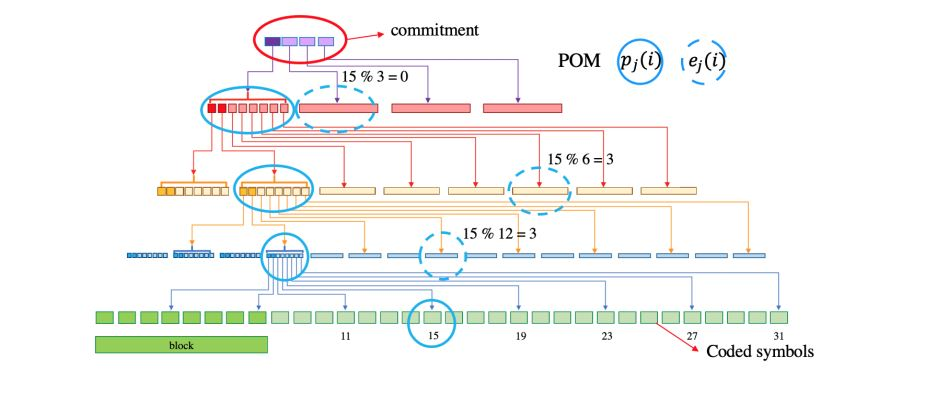
\includegraphics[width=0.8\linewidth]{Fig/12/F2}
		\caption{(1) CIT construction process of a block with $s\ell = 8$ data symbols, applied with erasure codes of coding ratio r = $\frac{1}{4}$. The batch size q = 8 and the number of hashes in root is t = 4. (2) Circled symbols constitute the $15$th base layer coded symbol and its POM. The solidly circled symbols are the base layer coded symbol and its Merkle proof (intermediate data symbols), the symbols circled in dash are parity symbols sampled deterministically.
		}
		\label{fig:L12_f2}
	\end{figure}
\end{center}
For all layers j except for the root, where $1 \leq j \leq \ell$, let's denote the set of all $m_{j}$ coded symbols as $M_{j}$. This set can be divided into two disjoint subsets of symbols: data symbols, represented as $S_{j}$, and parity symbols, represented as $P_{j}$. The count of data symbols is $s_[j] = rm_{j}$, and they are specified as $Sj = [0, rm_{j})$. On the other hand, the parity symbols are specified as $P_{j} = [rm_{j}, m_{j})$. For a given block containing $s_{\ell}$ data symbols in the base layer, the aggregation rule for the $k$-th data symbol in layer $j - 1$ is defined as follows:
\begin{equation} 
	Q_{j-1}[k] = \{(H(M_{j}[x])) | x \in [0, M_{j}), k = x \mod rm_{j - 1}\}
\end{equation}
\begin{equation} 
	M_{j-1}[k] = H(\text{concat}(Q_{j-1}[k])) 
\end{equation}
In the above equations, $1 \leq j \leq \ell$, and H denotes a hash function. The tuple Q[k] comprises hashes that will be utilized to generate the k-th symbol in the parent layer. Additionally, the function concat signifies the process of string concatenation, which involves combining all elements within an input tuple. This procedure remains consistent with the formulas provided earlier.\\

\renewcommand{\bibname}{References}
\begin{thebibliography}{9}
	\bibitem{reference1} Mustafa Al-Bassam, Alberto Sonnino, and Vitalik Buterin. Fraud and data availability proofs: Maximising light client security and scaling blockchains with dishonest majorities. \textit{arXiv preprint arXiv:1809.09044, 2018}
	\bibitem{reference2} Shu Lin and Daniel J Costello. \textit{Error control coding}, volume 2. Prentice hall, 2001.
	\bibitem{reference3} Irving S Reed and Gustave Solomon. Polynomial codes over certain fnite felds. \textit{Journal of the society for industrial and applied mathematics}, 8(2):300–304, 1960.
	\bibitem{reference4} Mingchao Yu, Saeid Sahraei, Songze Li, Salman Avestimehr, Sreeram Kannan, and Pramod Viswanath. Coded merkle tree: Solving data availability attacks in blockchains. In \textit{International Conference on Financial Cryptography and Data Security}, pages 114–134. Springer, 2020.
\end{thebibliography}